\chapter{Installation and Setup}
What do you need in order to install the pyNE software package on a new computer? All the necessary installer files should be located in the 'Documentation/ Installers' directory.
\section{Prerequisites and installation}
\paragraph*{Anaconda}
We recommend using the \textbf{Anaconda 64-bit Python 3.7} distribution unless you are on an older machine running 32-bit OS. Anaconda contains almost all of the required scientific modules, e.g., \textit{numpy} and \textit{matplotlib} that pyNE requires internally to function. Smaller builds such as Miniconda, won't have these. There shouldn't be any 64-bit compatability issues unless you are using either very ancient NI GPIB hardware or an OS that doesn't support 64-bit. In either of these instances, you may want to return to pyNE for python 2.7 (original build).\\
\\
The Anaconda download will be an executable that will install the software in your system. You can find it at: https://www.anaconda.com/distribution/ but be sure to download the windows version (the page there tends to default to MacOS as the download). Follow the prompts, and run with its default options, it should be pretty straightforward. It is a good idea to install `for all users' if asked to ensure portability across users on the same machine. Once it is installed, you should reboot your system to ensure the environment \& dependencies are correctly set-up. Note: you can delay this reboot until after the next step if you need to install NI-VISA also.\\

\paragraph*{National instruments (NI) VISA libraries and drivers}
If these are not already on your machine, you will need to download and install these also. These can be found here: https://www.ni.com/en-au/support/downloads/drivers/download.ni-visa.html\#305862 We recommend installing as 64-bit unless your OS is still 32-bit or you are using extremely old NI hardware. Install using defaults, it is rather straightforward. After this step you should reboot your system to ensure the environment \& dependencies are correctly set-up.\\

\paragraph*{Install pyVisa and nidaq-mx libraries for python}
There are two python libraries that aren't in the standard Anaconda distribution that we need to add. The first is the python libraries for running NI Visa. The second are the libraries specific to the USB-6216 can National Instruments MAX (NI-MAX). The latter actually has two options, PyDAQmx and nidaqmx python API. I chose the latter as it's written/supported by NI, but if you want to use the former, you need to install that library using the same method below.
\begin{enumerate}
\item In the windows start screen search for 'Anaconda prompt'.
\item Right click on it and choose the 'Run as Administrator' option, then select yes when the OS acts you to confirm you want to run as admin. You need to use this option here, or the library install may fail due to access block issues.
\item A terminal should appear. To install pyVisa, type '\texttt{conda install -c conda-forge pyvisa}' and execute. This should automatically install the module with all its dependencies.
\item After this completes, follow up with '\texttt{conda install -c conda-forge nidaqmx}' to install the NIDAQ libraries. If you want PyDaqmx, you will need to install using pip as it's not presently supported by Conda-forge. You might want to talk to Adam about some of the issues here before proceeding.
\end{enumerate}

\paragraph*{Creating a base folder/path}. pyNE itself is only a collection of scripts and thus does not need to be installed as such. You just choose a suitable folder and copy the contents of the latest pyNE version into it. Write down the full path of this folder. Every \textit{control file} starts with importing these scripts via
\begin{verbatim}
import os
os.chdir('basefolder')
from Imports import *
\end{verbatim}
and you need to use the filepath where your pyNE scripts are located.

\paragraph*{Spyder IDE}
This is automatically installed with Anaconda. You run it from the same Anaconda prompt that you used to install the pyvisa and nidaqmx libraries (you don't need to be admin to run it, only for package installations). To do this, you type '\texttt{spyder}' and it should start up. An example screenshot is shown below.\\

\begin{figure}[h]
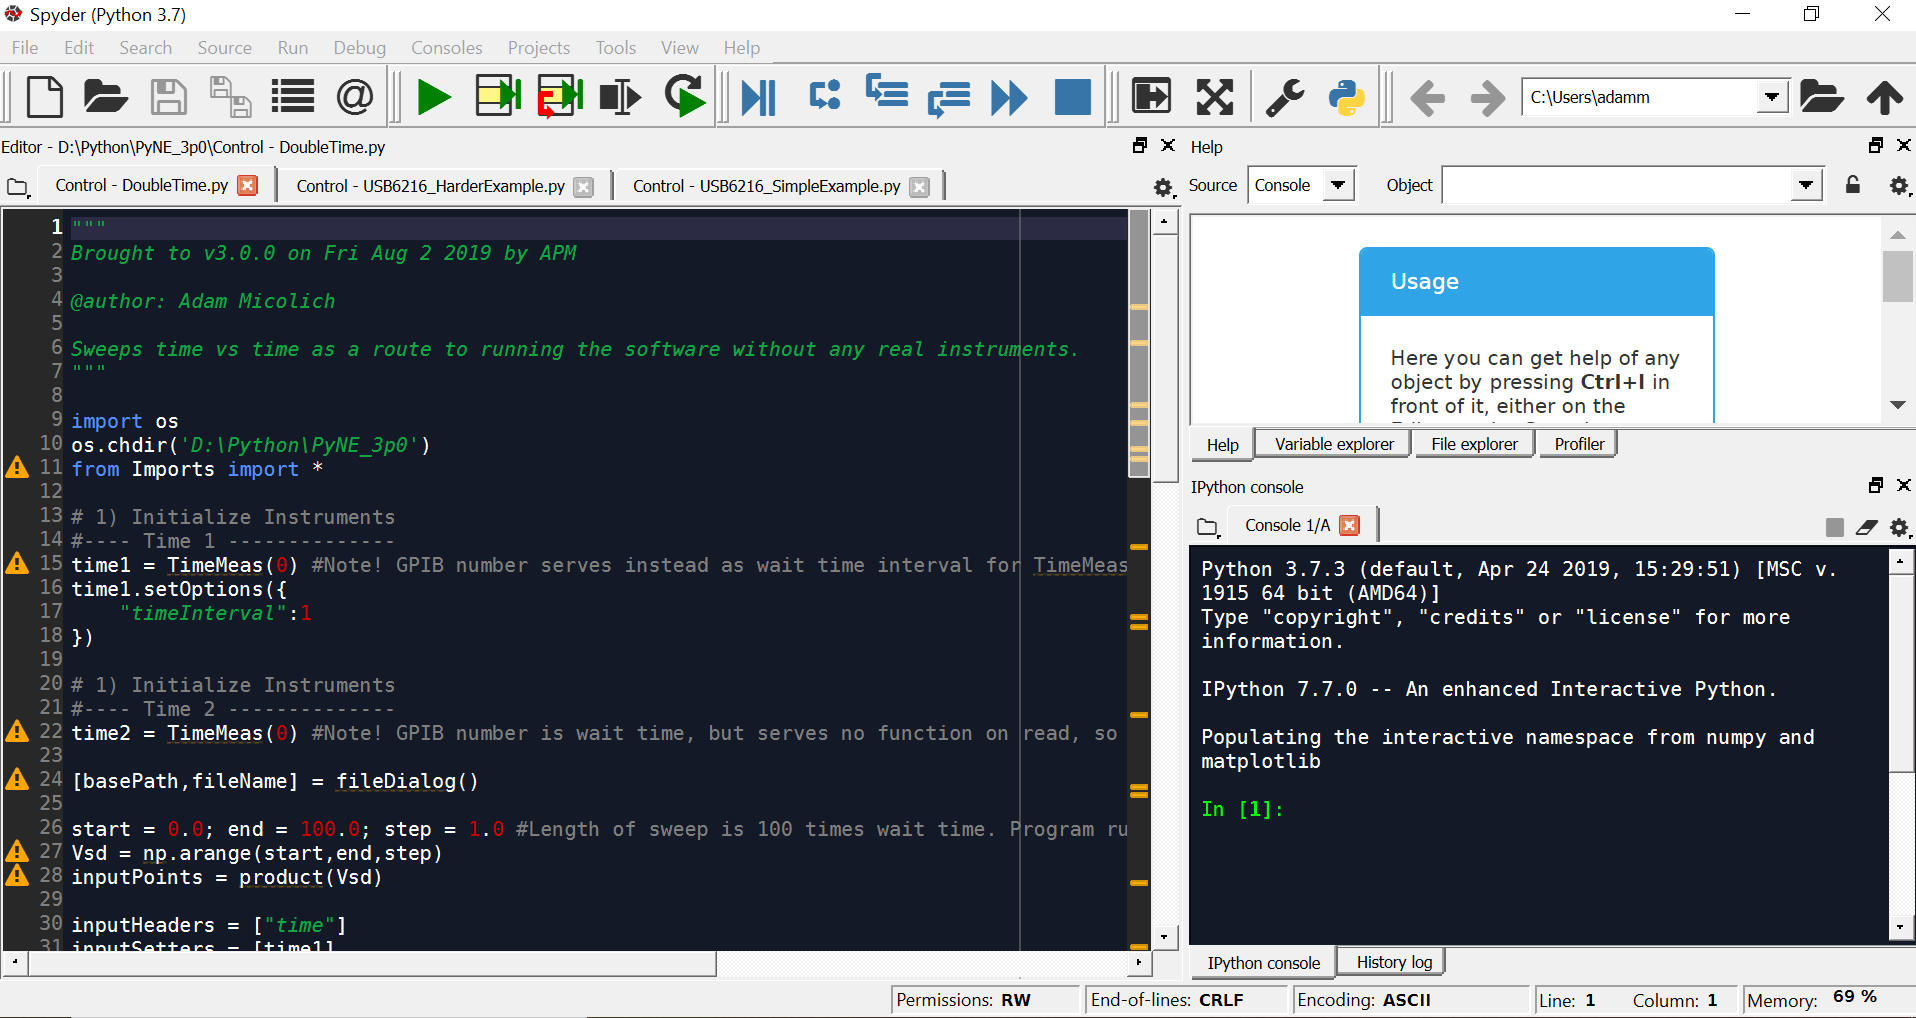
\includegraphics[width=16cm]{Spyder_screen}
\caption{\textbf{Spyder screenshot} Programs are loaded and edited on the left, the bottom right is your iPython console for running commands and seeing program output, the top right has panels for looking at contents of program variables, file structures, etc.}
\label{Fig:Spyderscreen}
\end{figure}

Figure~\ref{Fig:Spyderscreen} shows a screenshot of the Spyder IDE. You load your relevant control file, edit accordingly (even if it's just to set the operating directory), save and then execute using the green triangle in the top menu (run). A good test for this is to use the Control - DoubleTime.py file in the Examples directory, it is designed to be run on a computer without any instruments attached, since it uses the TimeMeas virtual instrument as both the control (setter) and output (reader) for the sweep. If it is working correctly, it should first bring up the GUI asking where to save the data file (see Section~1), and then put a graph to screen plotting time against time (trivial I know, but a good test for correct installation) and terminate.

\paragraph*{Setup the proper measurement ID file.}
Every measurement in pyNE has a running script consisting of a two letters and increasing number. For example, MeasurementNamePr123 would mean that the measurement 'MeasurementName' (which it takes from the GUI that comes up when you start a sweep) was the 123rd measurement on the Rack that is associated with the measurement setup Pr (in this case the probestation/gasbox).\\
\\
When initializing a new setup, we have to do two things: Set the counter back to zero and create a new letter combination associated with this new setup. To do this:\\
\begin{enumerate}
\item Open the GlobalMeasID.py file in spyder so you can edit its contents. Change the IDpath variable to 'basefolder\setminus GlobalMeasIDBinary'. Edit the \texttt{currentSetup} variable to a string of your choice. We recommend keeping it down to two letters for simplicity, e.g., 'Pr' for Probestation as in the example code.
\item Import GlobalMeasID in Spyder so you can access its functions in the console. If Spyder can't locate it, change the current working directory into your pyNE folder. Now execute GlobalMeasID.init(). This will set the internal counter to zero.
\end{enumerate}

An alternative way to set the counter to zero is just to open the GlobalMeasIDBinary file using Spyder and change the number to zero and then save. 